\documentclass[11pt]{article}

% load some asm stuff -
\usepackage{amssymb}
\usepackage{amsmath}
\usepackage{amsthm}
%\usepackage{palatino,lettrine}
\usepackage{fancyhdr}
\usepackage{epsfig}
\usepackage[round,comma,sort]{natbib}
\usepackage{simplemargins}
\usepackage{setspace}
\usepackage{boiboites}
\usepackage[margin=0pt,font=small,labelfont=bf]{caption}

\bibliographystyle{plos2009}

% Set the size
%\textwidth = 6.75 in
%\textheight = 9.75 in
%\oddsidemargin = 0.0 in
%\evensidemargin = 0.0 in
%\topmargin = 0.01 in
%\headheight = 0.0 in
%\headsep = 0.25 in
%\parskip = 0.15in
\doublespace

\setallmargins{1in}

\newtheorem{example}{Example}
\newtheorem{example*}{Example}
\newtheorem{thm}{Theorem}[section]
\newtheorem{property}{Property}[section]

\theoremstyle{definition}
\newtheorem{defn}[thm]{Definition}

\makeatletter
\renewcommand\subsection{\@startsection
	{subsection}{2}{0mm}
	{-0.05in}
	{-0.5\baselineskip}
	{\normalfont\normalsize\bfseries}}
\renewcommand\subsubsection{\@startsection
	{subsubsection}{2}{0mm}
	{-0.05in}
	{-0.5\baselineskip}
	{\normalfont\normalsize\itshape}}
\renewcommand\paragraph{\@startsection
	{paragraph}{2}{0mm}
	{-0.05in}
	{-0.5\baselineskip}
	{\normalfont\normalsize\itshape}}
\makeatother
\linespread{1.2}

\fancypagestyle{proposal}{\fancyhf{}%
	\fancyhead[RO,LE]{\thepage}%
	\fancyhead[LO,RE]{ChE 525 Intracellular metabolic networks}%
	\renewcommand\headrulewidth{1pt}}
\pagestyle{proposal}

% Single space'd bib -
\setlength\bibsep{0pt}

\renewcommand{\rmdefault}{phv}\renewcommand{\sfdefault}{phv}

\newboxedtheorem[boxcolor=black, background=gray!5,titlebackground=orange!20,titleboxcolor = black]{color_box_example}{Example}{test}

% Change the number format in the ref list -
\renewcommand{\bibnumfmt}[1]{#1.}

% Change Figure to Fig.
\renewcommand{\figurename}{Fig.}

%Joycelyn Chan, Joshua Lequieu, Michael Paull, Chidanand Balaji, Ryan Tasseff
%Our derivation follows closely the earlier development of Fredrickson \citep{Fredrickson:1976fk}.

% Begin ...
\begin{document}

%\begin{titlepage}
{\par\centering\textbf{\Large Intracellular Metabolic Networks and Flux Balance Analysis}}
\vspace{0.2in}
{\par \centering \large{Jeffrey D. Varner$^{*}$}}
\vspace{0.05in}
{\par \centering \large{School of Chemical Engineering$^{*}$}}
{\par \centering \large{Purdue University, West Lafayette IN 47907}}
\vspace{0.1in}
{\par \centering \small{Copyright \copyright\ Jeffrey Varner 2016. All Rights Reserved.}}\\

%\end{titlepage}
\date{}
\thispagestyle{empty}

\setcounter{page}{1}

%material and energy balances around the different processes cells do. For example, understanding how the abundance of raw materials in a bioreactor influences
%cell growth, or the production of valuable protein or small molecule products requires a materials balances around the major components of the system.
%The production of valuable small molecule or protein products requires large connected intracellular reaction networks that produce or consume energy.
%Thus, to understand the operation of biochemical systems and ultimately to manipulate them for societal gain,

%We developed material balances for nutrients, products and cells for batch, fed-batch and continuous stirred tank bioreactors.
%We also considered the \textit{best} way to operate bioreactors, for example, to maximize the amount of the product or
%the rate of product production in a given time period by varying process parameters, such as volumetric flow rate.
%However, we have not considered the problem of changing the \textit{intracellular} operation of cells.

\section*{Introduction}
Cells operate vast interconnected biochemical \textit{networks} to process starting materials such as sugars into valuable products of interest, waste products and eventually more cells.
To start exploring metabolic networks, lets first write material balances
around the reactants and products being consumed or produced by the enzymes (catalytic protein) in these networks.

\subsection*{General intracellular species balance equations.}
To derive the material balance governing the specific intracellular concentration of the $j^{th}$ metabolite $x_{j}$ ([mmol/gdw]) in a metabolic network,
we start from the general material balance:
\begin{equation}\label{eqn:general-balances}
\dot{n}_{X,acc,j} = \dot{n}_{X,in,j} - \dot{n}_{X,out,j} + \dot{n}_{X,gen,j}\qquad{j=1,2,\hdots,\mathcal{M}}
\end{equation}where $\mathcal{M}$ denotes the number of metabolites and X denotes a specific cell from our population of cells.
However, we have millions of cells in a bioreactor. Thus, we can't track metabolite levels in each individual cell.
Instead, we make the well mixed assumption (WMA) for the cells in the reactor. The WMA for cells implies that
the intracellular level of the metabolite $x_{j}$ does not vary between cells i.e., if we sample $x_{j}$ in many cells, the levels of $x_{j}$ would
be the same to within measurement error. Second, WMA also implies that $x_{j}$ does not vary with position \emph{inside} the cells.
In reality, the WMA assumption for cells is incorrect;
there are many interesting phenomena (both technological and human health related) that occur because of cellular diversity.
Moreover, it is well known (especially in eukaryotes) that the abundance of metabolites varies between the different cellular compartments.
However, for now we'll make this assumption.

There are only two terms that we need to consider for intracellular balances, the accumulation and generation terms.
This is because there is no \emph{convective} transport into or from the cellular phase, i.e., cell walls block convective transport of $x_{j}$
into or from the cell. Thus, the transport terms vanish $\dot{n}_{X,in,j} = \dot{n}_{X,out,j} = 0$ and the intracellular material balance around
metabolite $x_{j}$ becomes:
\begin{equation}\label{eqn:general-balances-no-transport}
\dot{n}_{X,acc,j} = \dot{n}_{X,gen,j}\qquad{j=1,2,\hdots,\mathcal{M}}
\end{equation}
The well-mixed assumption simplifies the accumulation term:
\begin{equation}\label{eqn-accumulation}
\dot{n}_{X,acc,j} = \frac{d}{dt}\int_{X}x_{j}dX\simeq X\frac{dx_{j}}{dt} + x_{j}\frac{dX}{dt}
\end{equation}while the generation term becomes:
\begin{equation}\label{eqn-generation}
\dot{n}_{X,gen,j} = \int_{X}\left(\displaystyle\sum_{r}^{\mathcal{R}}\sigma_{jr}v_{r} + \displaystyle\sum_{k}^{\mathcal{T}}\tau_{jk}q_{k}\right)dX \simeq \left(\displaystyle\sum_{r}^{\mathcal{R}}\sigma_{jr}v_{r} + \displaystyle\sum_{k}^{\mathcal{T}}\tau_{jk}q_{k}\right)X
\end{equation}We have split the reaction rates into those rates that occur completely within cells ($v_{k}'s$) and those that cross the cell boundary
($q_{k}'s$) where $\sigma_{jr}$ and $\tau_{jk}$ denote the respective stoichiometric coefficients.
These rates, called \textit{metabolic~fluxes}, have a special unit system called specific units.
The most used example of specific units for fluxes is [mmol/gdw-hr], however other examples are possible.
In general, metabolic fluxes are complex functions of the concentration of the enzymes that catalyze the reactions (intracellular protein catalysts manufactured by cells),
as well as substrates (starting materials) and sometimes even the products of other reactions.
Substituting the accumulation and generation terms into
Eqn \eqref{eqn:general-balances-no-transport} gives:
\begin{equation}\label{eqn-almost}
X\frac{dx_{j}}{dt} + x_{j}\frac{dX}{dt} = \left(\displaystyle\sum_{r}^{\mathcal{R}}\sigma_{jr}v_{r} + \displaystyle\sum_{k}^{\mathcal{T}}\tau_{jk}q_{k}\right)X
\qquad{j=1,2,\hdots,\mathcal{M}}
\end{equation}Rearranging Eqn \eqref{eqn-almost} and dividing by the cellmass gives:
\begin{equation}\label{eqn-xjbalance}
\frac{dx_{j}}{dt} = \left(\displaystyle\sum_{r}^{\mathcal{R}}\sigma_{jr}v_{r} + \displaystyle\sum_{k}^{\mathcal{T}}\tau_{jk}q_{k}\right) - \frac{x_{j}}{X}\frac{dX}{dt}
\qquad{j=1,2,\hdots,\mathcal{M}}
\end{equation}The last term on the right-hand side of Eqn \eqref{eqn-xjbalance} is a dilution term.
This term accounts for the loss of $x_{j}$ because of the growth of the cellmass population.
The dilution term couples the intracellular metabolite balances to the extracellular cellmass balance in a bioreactor, and thus to the operation of the bioreactor.

Let's assume we are growing cells in a batch process. This assumption implies the dilution term can be re-written as:
\begin{equation}
\frac{x_{j}}{X}\frac{dX}{dt} = \mu x_{j}
\end{equation}where
\begin{equation}
\mu = \frac{1}{X}\frac{dX}{dt}
\end{equation}
Putting everything together, we arrive at the general intracellular material balance governing $x_{j}$ in index-form:
\begin{equation}\label{eqn-final-mass-balance}
	\frac{dx_{j}}{dt} = \left(\displaystyle\sum_{r}^{\mathcal{R}}\sigma_{jr}v_{r} + \displaystyle\sum_{k}^{\mathcal{T}}\tau_{jk}q_{k}\right) - \mu x_{j}
	\qquad{j=1,2,\hdots,\mathcal{M}}
\end{equation}or in matrix-vector:
\begin{equation}
	\frac{d\mathbf{x}}{dt} = \mathbf{S}\mathbf{v} + \mathbf{T}\mathbf{q} -\mu\mathbf{x}
\end{equation}where $\mathbf{x}$ denotes the species abundance vector ($\mathcal{M}\times{1}$), $\mathbf{S}$ denotes the stoichiometric matrix ($\mathcal{M}\times{\mathcal{R}}$),
$\mathbf{T}$ denotes the transport (or exchange) matrix ($\mathcal{M}\times{\mathcal{T}}$) and the $\mathbf{I}$ denotes the ($\mathcal{M}\times{\mathcal{M}}$) identity matrix.

\begin{figure*}[h!]\centering
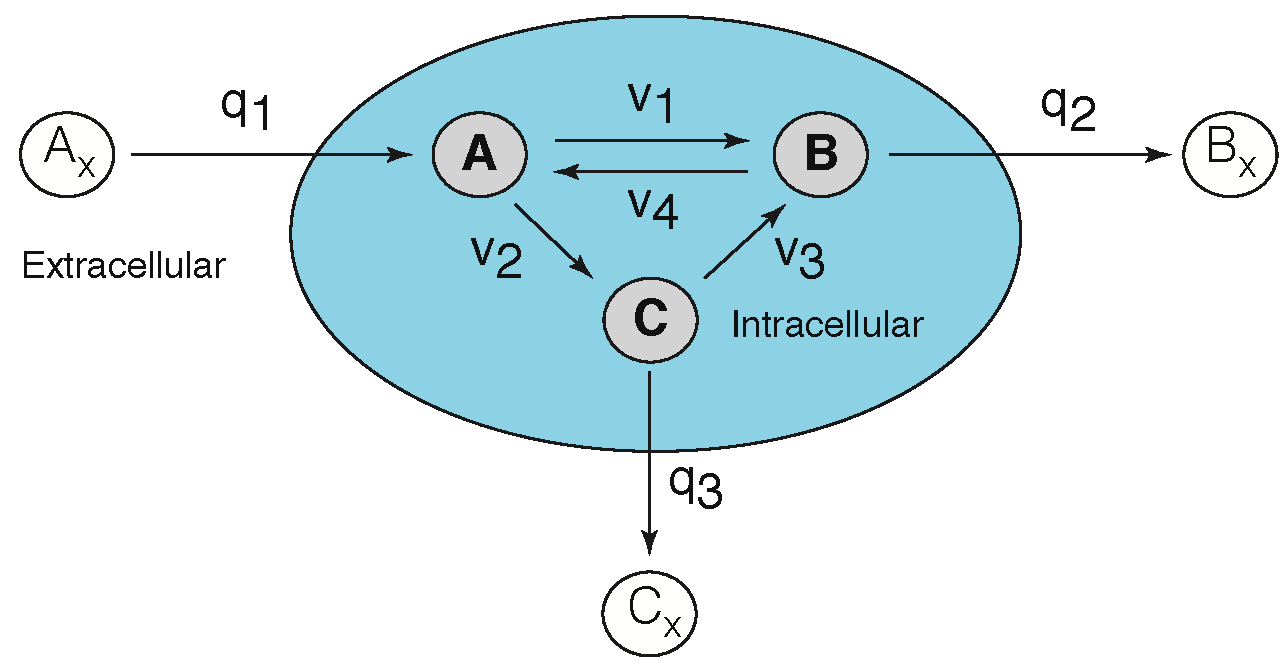
\includegraphics[,width=0.9\textwidth]{./figs/Simple-network-example.pdf}
\caption{Schematic of simple metabolic reaction network. This system has a total of six metabolites and seven reactions. The intracellular metabolites (metabolites $A,B$ and $C$) are often treated as balanced (no accumulation) while the extracellular metabolites ($A_{x},B_{x}$ and $C_{x}$) are not conserved (can accumulate). The blue-oval denotes the cell boundaries, where $q_{j}$ denotes flux across these boundaries ([mmol/gdw-hr]) and $v_{k}$ denotes the intracellular fluxes.}\label{fig-system}
\end{figure*}

\subsubsection*{Example: Formulate model system.}Formulate the intracellular metabolite balances for the network shown in Fig. (\ref{fig-system}). The example network has a total of six metabolites and seven reactions. The metabolites $A,B$ and $C$ are intracellular (inside the cell), while $A_x,B_x$ and $C_x$ are extracellular (outside the cell). Using the general intracellular species mass balance formulation (and neglecting the dilution due to growth terms) yields the material balances:
	\begin{equation}\label{eqn-full-system}
		\displaystyle\begin{bmatrix}
			\frac{dA}{dt} \\
			\frac{dB}{dt} \\
			\frac{dC}{dt} \\
		\end{bmatrix} =
		\begin{bmatrix}
			-1 & -1 & 0 & 1 & 1 & 0 & 0 \\
			1 & 0 & 1 & -1 & 0 & -1 & 0 \\
			0 & 1 & -1 & 0 & 0 & 0 & -1 \\
		\end{bmatrix}\cdot
		\begin{bmatrix}
			v_{1} \\
			v_{2} \\
			v_{3} \\
			v_{4} \\
			q_{1} \\
			q_{2} \\
			q_{3}
		\end{bmatrix}
	\end{equation}
	The material balances can be rewritten in matrix vector form:
	\begin{equation}
		\frac{d\mathbf{x}}{dt} = \mathbf{S}\mathbf{v} + \mathbf{T}\mathbf{q}
	\end{equation}where $\mathbf{x}\equiv\left\{A,B,C\right\}^{T}$, the intracellular flux vector is defined as
	$\mathbf{v} \equiv \left\{v_{1},v_{2},v_{3},v_{4}\right\}^{T}$ and the specific transport (exchange) vector is defined as $\mathbf{q} \equiv \left\{q_{1},q_{2},q_{3}\right\}^{T}$.
	The stoichiometric matrix $\mathbf{S}$ is then given by:
	\begin{equation}\nonumber
		\mathbf{S} \equiv
		\begin{bmatrix}
			-1 & -1 & 0 & 1 \\
			1 & 0 & 1 & -1 \\
			0 & 1 & -1 & 0 \\
		\end{bmatrix}
	\end{equation}while the transport or exchange matrix $\mathbf{T}$ is given by:
	\begin{equation}\nonumber
		\mathbf{T} \equiv
		\begin{bmatrix}
			1 & 0 & 0 \\
			0 & -1 & 0 \\
			0 & 0 & -1 \\
		\end{bmatrix}
	\end{equation}

\subsubsection*{Why did we neglect the $\mu x_{j}$ terms?}
Most researchers in the systems biology community neglect intracellular metabolite dilution terms because they are small relative to the
magnitudes of the reaction and transport fluxes ($v_{k}\sim q_{t}\gg\mu x_{j}$).
Additionally, they frustrate the mathematical analysis of intracellular networks using
approaches such as Flux Balance Analysis (FBA) as described by Palsson and coworkers \citep{Orth:2010uq}.
However, the shrinking and often marginalized kinetic modeling community still includes these terms
because they modify intracellular concentration, and thus the reaction kinetics encoded in the $v_{k}$'s and $q_{k}$'s.
These terms follow from the classic work of Fredrickson \citep{Fredrickson:1976fk} who showed they can be important in some cases.

\subsection*{What can we learn from the structure of a metabolic system?}
We can calculate interesting properties about a metabolic system by analyzing the structure of the stoichiometric and transport matrices.
Starting from the binary form of the augmented matrix (only entries in the matrices or 0 and 1):
\begin{equation}
	\mathcal{S} \equiv \Bigl[\hat{\mathbf{S}}\Bigr|\hat{\mathbf{T}}\Bigr]
\end{equation}
where $\hat{\mathbf{S}}$ and $\hat{\mathbf{T}}$ denote the stoichiometric and transport arrays with all non-zero terms replaced by 1.
The participation number for reaction $j$, defined as the number of metabolites that participate in reaction $j$, is given the symbol $\pi_{j}$ and defined as:
\begin{equation}
	\pi_{j} \equiv \sum_{i = 1}^{\mathcal{M}}\mathcal{S}_{ij}\qquad j = 1,2,\dots,\mathcal{R} + \mathcal{T}
\end{equation}while the connectivity number $\rho_{i}$, defined as the number of reactions that a metabolite participates in, is defined as:
\begin{equation}
	\rho_{i} \equiv \sum_{j = 1}^{\mathcal{R} + \mathcal{T}}\mathcal{S}_{ij}\qquad i=1,2,\dots,\mathcal{M}
\end{equation}
We can also learn about the extent of cross talk in a network by
analyzing the compound adjacency ($\mathcal{A}_{x} = \mathcal{S}\mathcal{S}^{T}$) and the reaction adjacency ($\mathcal{A}_{r} = \mathcal{S}^{T}\mathcal{S}$) arrays.
The diagonal elements of $\mathcal{A}_{x}$ give the number of reactions in which compound $x_{i}$ participates (the connectivity number),
while the off diagonal elements give the number of reactions in which both compounds $x_{i}$ and $x_{j}$ participate.
One the other hand, the diagonal elements of $\mathcal{A}_{r}$ give the participation number and the off diagonal elements
quantify how many compounds two reactions have in common.

\subsubsection*{Example: Analyze the structure of a metabolic network.}
Analyze the structure of the metabolic network shown in Fig. (\ref{fig-system}).
The augmented binary array for this network is given by:
\begin{equation}
	\mathcal{S} =
	\begin{bmatrix}
		1 & 1 & 0 & 1 & 1 & 0 & 0 \\
		1 & 0 & 1 & 1 & 0 & 1 & 0 \\
		0 & 1 & 1 & 0 & 0 & 0 & 1 \\
	\end{bmatrix}
\end{equation}
The metabolite and reaction adjacency arrays are given by:
\begin{equation}
	\mathcal{A}_{x} =
	\begin{bmatrix}
		4  & 2 &  1 \\
		2  &  4 &  1 \\
	   	1  &  1  & 3 \\
	\end{bmatrix}
\end{equation}and
\begin{equation}
	\mathcal{A}_{r} =
	\begin{bmatrix}
		   2 &  1  &  1 &  2  & 1  & 1  & 0 \\
		   1 &  2  &  1 &  1  & 1  & 0  & 1 \\
		   1 &  1  &  2 &  1  & 0  & 1  & 1 \\
		   2 &  1  &  1 &  2  & 1  & 1  & 0 \\
		   1 &  1  &  0 &  1  & 1  & 0  & 0 \\
		   1 &  0  &  1 &  1  & 0  & 1  & 0 \\
		   0 &  1  &  1 &  0  & 0  & 0  & 1 \\
	\end{bmatrix}
\end{equation}respectively. From these arrays we can estimate connectivity and crosstalk information about the metabolic network.

\subsection*{Flux balance analysis (FBA).}
Flux balance analysis (FBA) is a strategy to estimate intracellular fluxes given a model of the metabolic network, and information about the rate of material exchange between
cells and the extracellular environment.
Flux balance analysis was developed by Palsson and coworkers to estimate fluxes of genome scale models of \emph{E. coli} \citep{Edwards:2000yq}.
The FBA problem recasts the estimation of intracellular fluxes as a Linear Programming (LP) problem.
Linear programming is a type of convex optimization problem in which a linear objective function is maximized (or minimized) subject to linear algebraic constraints.
LPs can be solved easily for genome scale problems with thousands of unknown fluxes on standard hardware using packages such as MATLAB in a few seconds.
The general form for a metabolic FBA problem is given by:
\begin{equation}
	\max_{\mathbf{v}}\mathbf{c^{T}}\mathbf{v}
\end{equation}
subject to the algebraic constraints:
\begin{eqnarray}
	\mathbf{S}\mathbf{v} + \mathbf{T}\mathbf{q} &\leq& \mathbf{b} \\
	\mathbf{v},\mathbf{q}&\geq&\mathbf{0}
\end{eqnarray}
where $\mathbf{c}^{T}$ is the \textit{objective selection vector} and $\mathbf{b}$ denotes the time-derivative vector for all system states (intracellular and extracellular), while
$\mathbf{S}$ and $\mathbf{T}$ denote the stoichiometric and transport arrays for both intracellular and extracellular metabolites (rows) for unmeasured and measured fluxes (columns).

\subsubsection*{Example: Simple flux balance analysis problem.}
	Estimate the intracellular fluxes for the simple reaction network shown in Fig. \eqref{fig-system} using flux balance analysis (FBA).
	FBA requires that we choose an objective vector, so lets assume we want to
	minimize $C_{x}$ production. This objective implies $\mathbf{c}^{T}$ = $\left(0,0,0,0,-1,0,0\right)$.
	Assuming we measured constrained $0\leq\dot{A}_{x}\leq{1}$ and $0\leq\dot{B}_{x}\leq{0.5}$,  we can redefine the stoichiometric and transport arrays as:
	\begin{equation}
	\mathbf{S} =
	\begin{bmatrix}
		-1 & -1 & 0 & 1 & 0 \\
		1 & 0 & 1 & -1 & 0 \\
		0 & 1 & -1 & 0 & -1 \\
		0 & 0 & 0 & 0 & 0 \\
		0 & 0 & 0 & 0 & 0 \\
		0 & 0 & 0 & 0 & 1 \\
	\end{bmatrix}
	\end{equation} and
	\begin{equation}
		\mathbf{T} =
		\begin{bmatrix}
			1 & 0 \\
			0 & -1 \\
			0 & 0 \\
			-1 & 0 \\
			0 & 1 \\
			0 & 0 \\
		\end{bmatrix}
	\end{equation}where the three extra rows are associated with the $A_{x}$, $B_{x}$ and $C_{x}$ balances.
	The minimum and maximum flux solutions for $C_{x}$ are given in Fig. \eqref{fig-fba-flux-solution}.


	\begin{figure*}[h!]\centering
	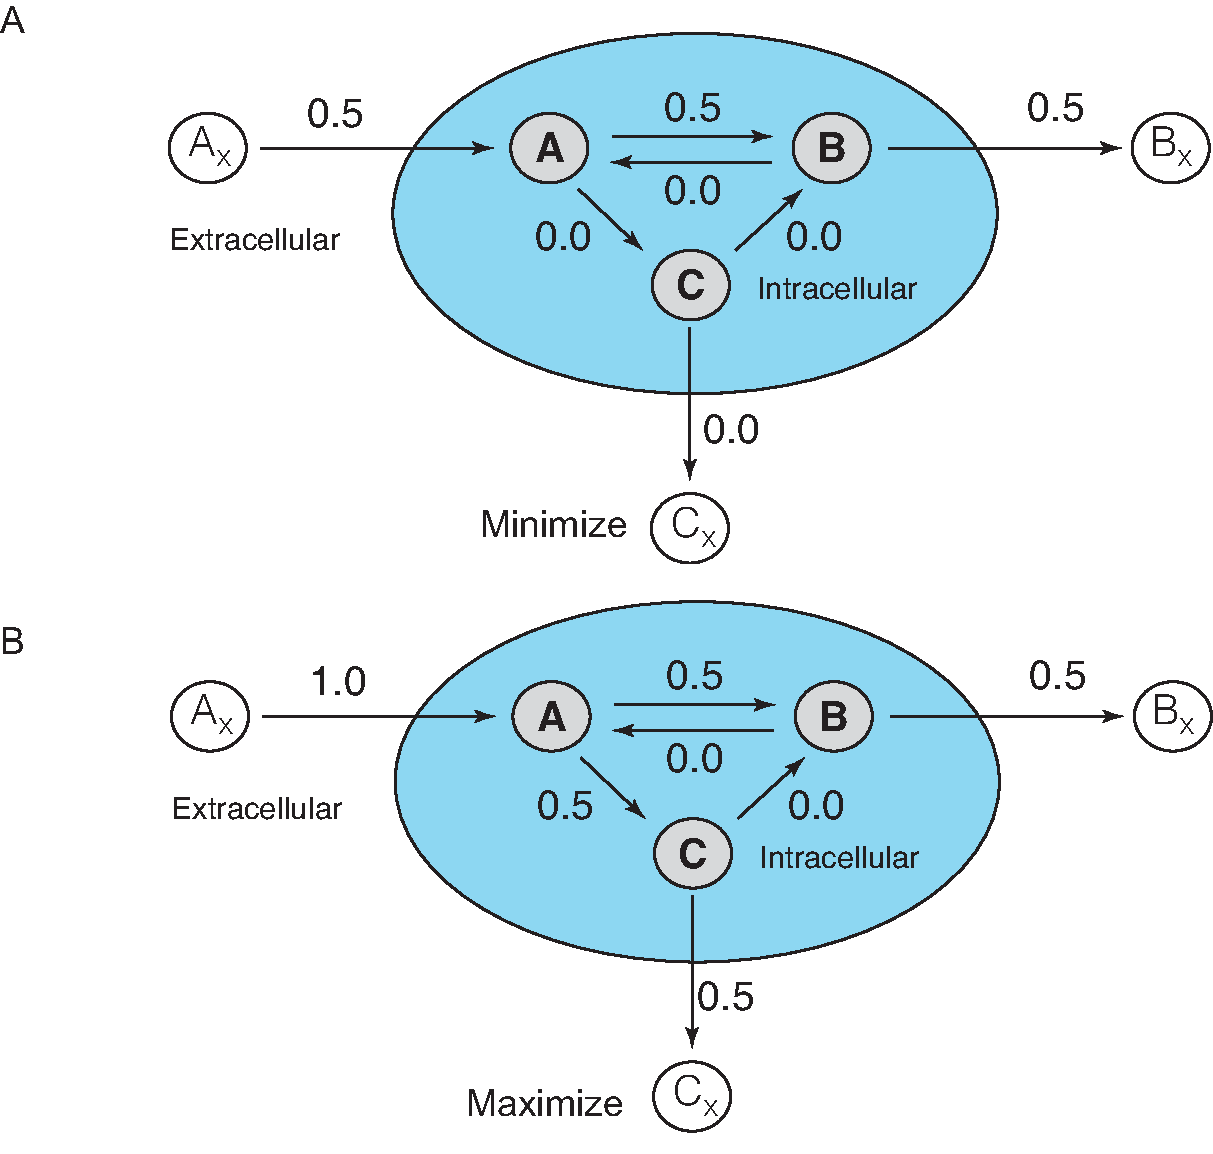
\includegraphics[,width=0.9\textwidth]{./figs/FBA-Solutions-Simple-Network.pdf}
	\caption{Example flux solution  $0\leq\dot{A}_{x}\leq{1}$ and $0\leq\dot{B}_{x}\leq{0.5}$ for minimizing or maximizing $C_{x}$.}\label{fig-fba-flux-solution}
	\end{figure*}

\clearpage

\bibliography{Notes}
\end{document}
